\section{Modeling}
\label{sec:singleActuator}
%
Our modeling approach for individual FREEs is based on the notion of a \emph{fluid Jacobian} $\bar{J}$, which maps the geometrical deformation of a soft actuator, or of a system of actuators, to a change in their volume. 
Under certain assumptions, the transpose of this Jacobian linearly maps the internal fluid pressure to the spatial forces that the actuator generates. 
One can  think of this fluid Jacobian as the soft and multi-dimensional equivalent of the cross section $A$ of a traditional pneumatic or hydraulic cylinder,
since this cross section similarly relates cylinder pressure to force, and piston movement to fluid displacement.


\subsection{Force Generation in a Single FREE}
%
The approach presented in this paper is enabled by a number of simplifying assumptions.
They are consistent with those made in prior work on the modeling and control of individual FREEs \cite{bishop2015design,bruder2017model}.
In particular, we assume that the fibers are inextensible and that they are uniformly  distributed  around  an elastomeric cavity  with negligible  wall thickness.
%The internal pressure in this cavity is uniform along its entire length.
Under these assumptions, a FREE can be modeled as a composition of an energy transforming element (the fibers) and an energy storing element (the compliance of the elastomer body). 
The generalized forces generated by each of these separate elements can be superimposed to characterize the net force $\vec{\tau}_{total}$ produced by the FREE:
\begin{align}
   \vec{\tau}_{\text{total}} &=  \vec{\tau} + \vec{\tau}_{\text{elast}}    \label{eq:netF}
\end{align}
where $\vec{\tau}$ and $\vec{\tau}_{\text{elast}}$ are the generalized forces and torques attributed to the fiber and elastomer, respectively.
In this work, we focus exclusively on the active general forces $\vec{\tau}$ that are generated by the fibers and that can be controlled by varying the pressure of the fluid.


The fluid Jacobian for such an actuator can be derived from the idea that the reinforcing fibers in a FREE create a kinematic constraint on the internal volume $V$ of the fluid cavity.
Without the reinforcing fibers, this cavity could expand freely, since it is made from soft material.
With the fibers, however, the volume is limited.
This limitation on volume depends on the mechanical parameters of the FREE (e.g., the relaxed fiber angle or fiber length) and on the current state of geometric deformation of the FREE.
This geometric state can be represented by a generalized vector of spatial deformations $\vec{q}$:  $V = V\left(\vec{q}\right)$.


The derivative of this volume yields an expression $\dot{V}$ for the volumetric flow into the actuator:
\begin{align}
    \dot{V} (\vec{q}, \dot{\vec{q}}) &= \frac{\partial V}{\partial t} = \frac{\partial V}{\partial \vec{q}} \frac{\partial \vec{q}}{\partial t } = \bar{J}_q (\vec{q}) \dot{\vec{q}},  \label{eq:Vdot_wJ}
\end{align}
where the fluid Jacobian is defined as $\bar{J}_{q}= \frac{\partial V}{\partial \vec{q}}$ with respect to the deformation $\vec{q}$. 


It is important to note that $\vec{\tau}$ and $\dot{\vec{q}}$ live in dual spaces. 
That is, forces in $\vec{\tau}$ correspond to linear motion in $\dot{\vec{q}}$, and moments in $\vec{\tau}$ correspond to angular motion in $\dot{\vec{q}}$.
In the most general case, these are 6-dimensional vectors with three translations and three rotations.
In this case, $\bar{J}_q$ is a $1 \times 6$ matrix.


Energy conservation dictates that the mechanical power generated by the fibers must equal the fluid power that goes into the FREE:
\begin{align}
    P_{\text{mech}} = P_{\text{fluid}} = \dot{\vec{q}}^{\,T} \vec{\tau} &= \dot{V} p, 
    \label{eq:Pequiv}
\end{align}
%
where $p>0$ is the pressure of the fluid inside the FREE.
Substituting \eqref{eq:Vdot_wJ} into \eqref{eq:Pequiv}, we arrive at a linear expression that yields the forces produced by the FREE fibers as a function of deformation state and fluid pressure: 
\begin{align}
    \vec{\tau} (\vec{q}, p) &= \bar{J}_q^T (\vec{q}) p       \label{eq:fiberF}
\end{align}
The fluid Jacobian thus describes the generalized direction in which a FREE can produce forces and torques.
Since the input pressure $p$ needs to be strictly positive to avoid collapsing of the fluid cavity, forces can only be produced in the positive direction defined by $\bar{J}_q$.


\subsection{The Fluid Jacobian of a Cylindrical FREE}
The theoretical modeling approach outlined above can be applied independently of the exact geometry of a FREE and can even be extended to other classes of soft actuators.
However, to make the computation of the fluid Jacobian tractable, we rely on another common assumption for FREES: that they maintain the geometry of an ideal cylinder \cite{bishop2015design}.
This neglects the tapering of the actuator towards the end-caps and any potential bending along its main axis.

\begin{figure}
    \centering
    \begin{tikzpicture}
        \node (FREEstate) at (0,0)
            {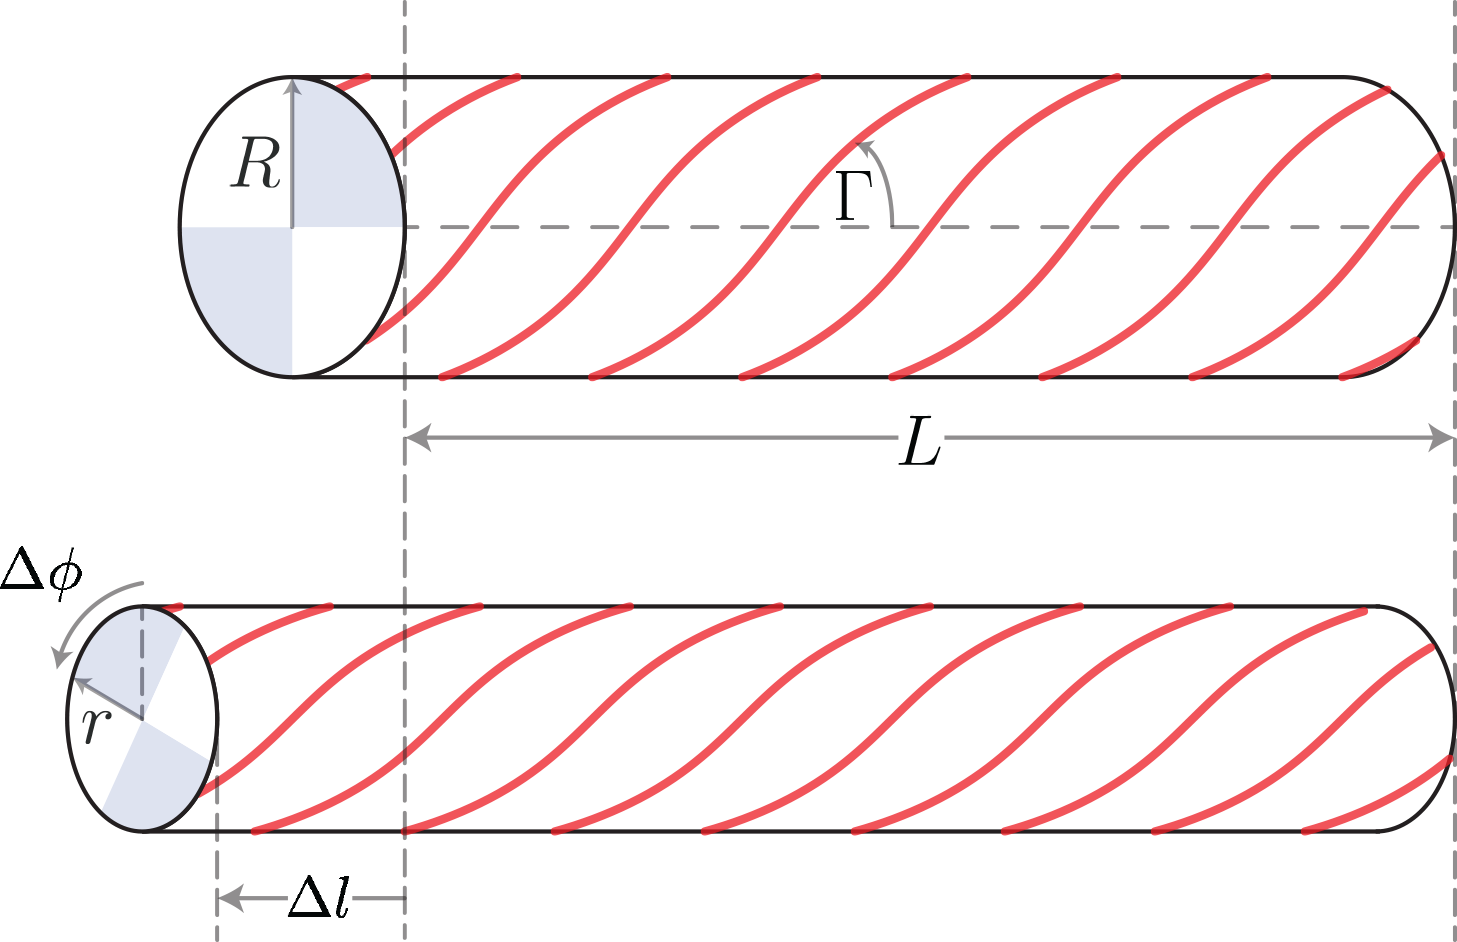
\includegraphics[width=0.75\linewidth]{figures/FREEstate_noLabels3.png}};
        \node[right] (a) at ($ (FREEstate.east) !0.5! (FREEstate.north east) $) {(a)};
        \node[right] (b) at ($ (FREEstate.east) !0.5! (FREEstate.south east) $) {(b)};
    \end{tikzpicture}
    \caption{Geometric parameters of an ideal cylindrical FREE in (a) the relaxed configuration where ${\vec{q}=0}$ (top), and (b) a deformed configuration where ${\vec{q} = \bmx \Delta l & \Delta \phi \emx^T}$ (bottom).}
    \label{fig:FREEparams}
\end{figure}

An ideal cylindrical FREE in its relaxed configuration (i.e. when gauge fluid pressure is zero and no external loads are applied) can be described by a set of three parameters, $L$, $R$, and $\Gamma$, where $L$ represents the relaxed length of the FREE, $R$ represents the radius, and $\Gamma$ the fiber angle (Fig.~\ref{fig:FREEparams}). 
For notational convenience, we define two other quantities from these parameters:
\begin{align}
	B &= \left| \frac{L}{\cos{\Gamma}} \right| \\
	N &= - \frac{L}{2 \pi R} \tan{\Gamma}
\end{align}
where $B$ is the length of one of the FREE fibers, and $N$ is the total number of revolutions the fiber makes around the FREE in the relaxed configuration. 

\revcomment{2.4}{The assumption that a FREE is cylindrical with inextensible fiber-reinforcements implies that changes in its radius, length, and twist are coupled 
% via the right triangle relationship shown in Fig. \ref{fig:fiber}
. Therefore, its geometrical deformation can be fully defined in terms of just two parameters, a change in its length $\Delta l$ and a twist about its main axis $\Delta \phi$.}
These two values constitute the vector of generalized deformations $\vec{q} = \left[ \Delta l, \Delta \phi \right]^T$.
Consequently the generalized torque vector $\vec{\tau} = \left[ F, M \right]^T$ describes a force along the main axis, $F$, and a torsional moment about that axis, $M$.

From this, the length and radius of the deformed FREE can be computed according to:
\begin{align}
    l &= L + \Delta l \label{eq:l} \\
	r &= \frac{B}{\abs{2 \pi N + \Delta \phi}} \sqrt{1 - \left( \frac{L+\Delta l}{B} \right)^2}, \label{eq:r}
\end{align}
and we can express the volume as
\begin{align}
	V(\vec{q}) &= \pi r^2 l \notag \\ 
	&= \frac{\pi (L+\Delta l) (B^2 - (L+\Delta l)^2)}{(2 \pi N + \Delta \phi)^2}  \label{eq:V}.
\end{align}

With this, the fluid Jacobian evaluates to:
\begin{align}
    \bar{J}_q (\vec{q})
    &= \begin{bmatrix} 
		        \frac{\pi \left( B^2 - 3(L + \Delta l)^2 \right)}{(2 \pi N + \Delta \phi)^2} & \frac{2 \pi (L+\Delta l) \left( (L+\Delta l)^2 - B^2 \right)}{(2 \pi N + \Delta \phi)^3}
		\end{bmatrix}.    \label{eq:Jv}
\end{align}


% % THIS FIGURE WILL BE REMOVED FOR SPACE IF NEEDED, BUT I WANT TO KEEP IT IF POSSIBLE 
% \begin{figure}
%     \centering
%     \begin{tikzpicture}
%         \node (fiber) at (0,0)
%             {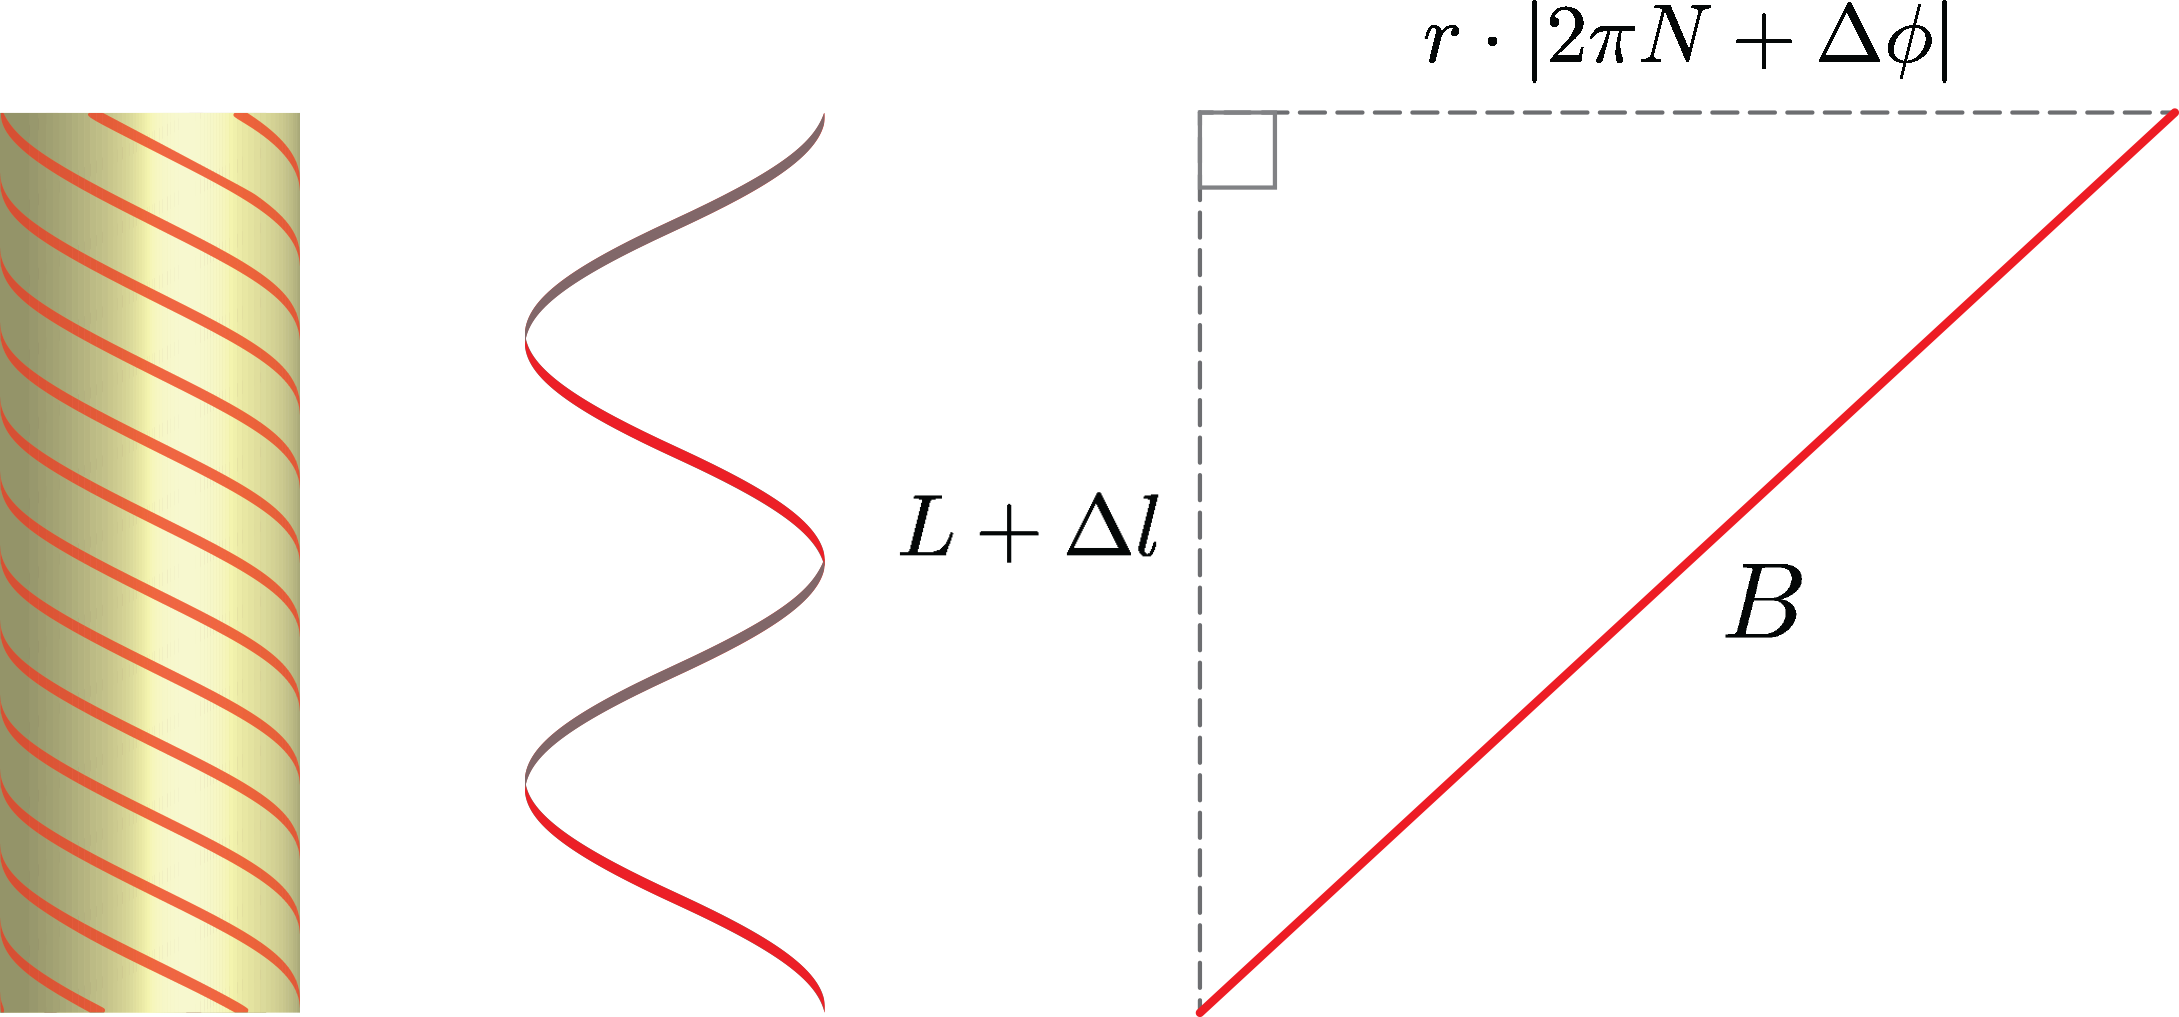
\includegraphics[width=0.85\linewidth]{figures/fiber_noLabels2.png}};
%         \node[below] (a) at ($ (fiber.south west) !0.08! (fiber.south east) $) {(a)};
%         \node[below] (b) at ($ (fiber.south west) !0.32! (fiber.south east) $) {(b)};
%         \node[below] (c) at ($ (fiber.south west) !0.75! (fiber.south east) $) {(c)};
%     \end{tikzpicture}
%     \caption{(a) A FREE contains many parallel fibers, all part of the same fiber family. (b) One isolated fiber forms a helical constraint. (c) The FREE radius $r$, twist $\Delta \phi$, and length change $\Delta l$ are geometrically related via the right triangle formed by unwinding a fiber and laying it flat.}
%     \label{fig:fiber}
% \end{figure}




